

%Set your metadata here:
\title{Implementing a \textcite{holt_risk_2002} Multiple Price List lottery in oTree}
\author{Olaf Ghanizadeh}


%
%
%  === PREAMBLE ============
%
% Define the document class 'book'.
% Set font size to 12, set to  A4 paper, and one-sided document.
\documentclass [12pt,a4paper,oneside]{article}

% Set font type to 'Times New Roman'.
\usepackage{times}

% Portuguese accents just in case.
\usepackage[T1]{fontenc}
\usepackage[utf8]{inputenc}

\usepackage[style=authoryear,backend=biber]{biblatex}

\addbibresource{progtech.bib}% Syntax for version >= 1.2

% English language.
\usepackage[english]{babel}

% appendix 
\usepackage[titletoc,toc,title]{appendix}
\newcommand{\nocontentsline}[3]{}
\newcommand{\tocless}[2]{\bgroup\let\addcontentsline=\nocontentsline#1{#2}\egroup}

\makeatletter

\def\@biblabel#1{\hspace*{-\labelsep}}

\makeatother

% Set margins to 3cm.
\usepackage[top=3cm, bottom=3cm, left=3cm, right=3cm]{geometry}

% Change margins command.
\def\changemargin#1#2{\list{}{\rightmargin#2\leftmargin#1}\item[]}
\let\endchangemargin=\endlist 

% Paragraph indentation.
\usepackage{indentfirst}
\usepackage{minted}

% Set vertical spacing to 1.5 lines.
\usepackage{setspace}
\onehalfspacing

\makeatletter
% Page headers and footers customisation.
\usepackage{fancyhdr}
\pagestyle{fancy}
\fancyhf{}
	% Set left header to footnotesize (10pt) and upper cases.
\lhead{\textsf{\scriptsize \textsc{\@author}}}
	% Set left header to footnotesize (10pt) and upper cases.
\rhead{\textsf{\scriptsize \textsc{\@title}}}
	% Set centred footer to page number.
\cfoot{\thepage}
\makeatother


% Customise chapters, sections, subsections, and subsubsections.
\usepackage{titlesec}
	% Set chapters' titles to upper cases and centred.
\titleformat{\chapter}[display]
  {\scshape\center}
  {}
  {0pt}
  {\thechapter.\ }
  \usepackage{etoolbox}% Stop chapters from starting at new page.
\makeatletter
\patchcmd{\chapter}{\if@openright\cleardoublepage\else\clearpage\fi}{}{}{}
\makeatother
	% Set sections' titles to upper cases and centred.
\titleformat{\section}
  {\scshape\center}{\thesection}{1em}{}
	% Set subsections' titles to italic and centred.
\titleformat{\subsection}
  {\itshape\center}{\thesubsection}{1em}{}
	% Idem for subsubsections' titles.
\titleformat{\subsubsection}
  {\itshape\center}{\thesubsection}{1em}{}


% Link objects (e.g. tables, figures, pages) in the body of text.
\usepackage{hyperref}

% Build a glossary.
%\usepackage{glossaries}
%\makeglossaries  
  % Define, e.g. acronyms (\newacronym{<label>}{<abbrv>}{<full>}).
  % Use \gls{<label>} command to call the acronym in the text. On first use the \gls command will display "<full> (<abbrv>)". On subsequent uses only the abbreviation will be displayed.



% Customize table of contents.
\usepackage{tocloft}
\setlength{\cftbeforetoctitleskip}{0pt}
%	\addto\captionsenglish{%
%	\renewcommand{\contentsname}{\hfill\normalfont\scshape\normalsize Table of Contents\hfill}   
	%\renewcommand{\cftaftertoctitle}{\hfill}
%	}

%\addto\captionsenglish{%
 % \renewcommand{\contentsname}%
  %  {\scshape Table of Contents}%
%}
\setlength{\cftbeforeloftitleskip}{0pt}
\setlength{\cftbeforelottitleskip}{0pt}

%Customise tables.
\renewcommand*\thetable{\Roman{table}}% Roman Numerals Tables
\addto\captionsenglish{\renewcommand{\tablename}{\textsc{Table}}}% Full Caps Tables
\addto\captionsenglish{\renewcommand{\figurename}{\textsc{Figure}}}% Full Caps Figures

%%%%%%%%%%%Tables
\usepackage{lipsum}

\usepackage{booktabs}
\usepackage{adjustbox}
\setlength\heavyrulewidth{0.3ex}

\usepackage{tabularx}
\usepackage{array}

\usepackage{threeparttable}


%Quotes
\usepackage{csquotes}




% Begin the document.
\begin{document}




%  = = = = = == = = = = = = Front and cover pages  = = = = = = = = = = == = =  

\makeatletter
\begin{titlepage}

\pagestyle{empty}
\centering

\begin{flushleft}
    
\includegraphics[width=0.3\linewidth]{graphics/Logotipo_ISEG.png}
\end{flushleft}    
    \vspace{3cm}
   {\textsf{\Huge Programming Techniques Project}} \\ [1cm]
    {\textsf{\Large 1º Sem. 2019/2020}} \\ [3cm]
  {\textsf{\Large \@title }} \\ [2cm] % <- delete the  irrelevant parts
%\begin{flushleft}
%{\uppercase{\Large \@title }} \\ [1.5cm] % <- write here the title of your thesis
%{\uppercase{\Large \@author }}  \\ [2cm]% <- write here the title of your thesis
%\end{flushleft}
\textsf{
\underline{Author:} \\
\@author}
    \vfill
%Date
    {\textsf{\Large ISEG, 10th  December 2019}}  % <- write here the date
 \clearpage 
 \end{titlepage}
 \makeatother



	\newpage % Create a new page.
	\thispagestyle{plain}% No header and footer.



\makeatletter	
\begin{center} % Begin centred text.


\textsc{\@title}\\ % Title of the dissertation.
    
By \@author \\
    

\end{center} % End centred text.
\makeatother

\section*{Abstract}


\section{Introduction}\label{sec:introduction}

This report explains the process of implementing a version of the Multiple Price List (MPL) lottery proposed in \cite{holt_risk_2002} in oTree, \textcite{chen_otreeopen-source_2016}, and the data...

By incentivizing participation in the experiment, participants are more likely to reveal their true risk preferences when compared with more traditonal methods such as questionaires. 
  


\section{Literature review}
The Multiple Price List approach popularized by \textcite{holt_risk_2002} has emerged as a simple, yet powerful framework for eliciting individual risk preferences and to estimate parameters of individual utility functions. As of December 2019, the paper has been cited more than 1900 times in the Web of Science \footnote{LINK} making it a tremendously influnetal paper in the domain of experimental and behavioral economics, whose methodology has been applied in a vast array of contexts. 


The work by \textcite{holt_risk_2002} has motivated the development of other methods to elicit personal risk preferences. \textcite{charness_experimental_2013-1} reviews some common methods of measuring individual risk preferences, where the MPL method is highlighted as a complex method. Complex meaning that it carries a risk of getting skewed results if participants do not understand the instructions of the experiment. In addition, if participants are allowed to switch between the alternatives freely, inconsistent results may be the result. \textcite{charness_experimental_2013-1} mentions a selection of studies where significant inconsistent behavior was recorded. 

\textcite{drichoutis_what_2016-2} argues that the \textcite{holt_risk_2002} method may not be the best approach to elicit risk preferences, and develops and extended version where the choices are made over a 





One key assumption in \textcite{holt_risk_2002} is that the theory of Constant Relative Risk Aversion holds (CRRA). 


Given this assumption





\section{Empirical Work}

\subsection{Experiment}
In this report I chose to employ a simplified version of the \textcite{holt_risk_2002} Multiple Price List Experiment. I decided to limit the experiment to one round and eight choices, thus, the value of the resulting data is limited. The decision to limit the lottery tho eight choices was made due to a technichal error arising if the tenth choice was randomly drawn by the computer. 
Additional simplifications were made in order to ensure that I was able to get my classmates to participate. 
Even though there was an incentive for participation in the experiment, they are not necessarily compatible, and the preferences revealed in the lotteries are therefore not robust. 

\paragraph{}
The experiment I asked my classmates to participate in had the following instructions:

\begin{quotation}
  
\subsection*{A Simple Lottery}
In this experiment you will take part in a lottery with the chance to win a prize. You will be presented with "Choices".

For each Choice you will pick an Option, A or B, which will give you two possibilities for winning a certain amount of points. When you are done, the computer will at random pick one of the Choices. Then the computer will check which Option you chose and draw your payoff according to the probability distribution of your picked Option in that Choice.

Before we start, please indicate your name, and tell us about your attitude towards risk.
\end{quotation}

The users were asked to enter their name for the purpose of drawing a prize during the presentation, and indicate their preferences for risk by choosing between the following alternatives:

\begin{enumerate}
  \item I prefer to avoid risks
  \item I am neutral towards risks
  \item I like taking risks if I can gain from it
\end{enumerate}

The next page consists of the choices the participants were asked to make. 

The choices and their respective payoffs and expected values are displayed in the table below. Where $p$ represents the probability of the high payoff being drawn, and $1-p$ the probability of the low payoff being drawn. 

The Difference column shows the difference between the expected value of chosing $A$ over $B$. Implying, that someone who is perfectly neutral towards risk would choose to switch from $A$ to $B$ at the 4th choice. 




\begin{table}[H]
  \centering
  \caption{Probabilities, choices and expected values}
    \begin{tabular}{ccccccccc}
      \toprule
         $p$ &  $1-p$ & $A_{High}$ & $A_{Low}$ & $B_{High}$ & $B_{Low}$ & $E[A]$ &   $E[B]$ & Difference \\
      \midrule
       0.125 &  0.875 &        200 &       160 &        385 &        10 &  165.0 &   56.875 &    108.125 \\
       0.250 &  0.750 &        200 &       160 &        385 &        10 &  170.0 &  103.750 &     66.250 \\
       0.375 &  0.625 &        200 &       160 &        385 &        10 &  175.0 &  150.625 &     24.375 \\
       0.500 &  0.500 &        200 &       160 &        385 &        10 &  180.0 &  197.500 &    -17.500 \\
       0.625 &  0.375 &        200 &       160 &        385 &        10 &  185.0 &  244.375 &    -59.375 \\
       0.750 &  0.250 &        200 &       160 &        385 &        10 &  190.0 &  291.250 &   -101.250 \\
       0.875 &  0.125 &        200 &       160 &        385 &        10 &  195.0 &  338.125 &   -143.125 \\
       1.000 &  0.000 &        200 &       160 &        385 &        10 &  200.0 &  385.000 &   -185.000 \\
      \bottomrule
    \end{tabular}
\end{table}

\begin{figure}[H]
  \centering
  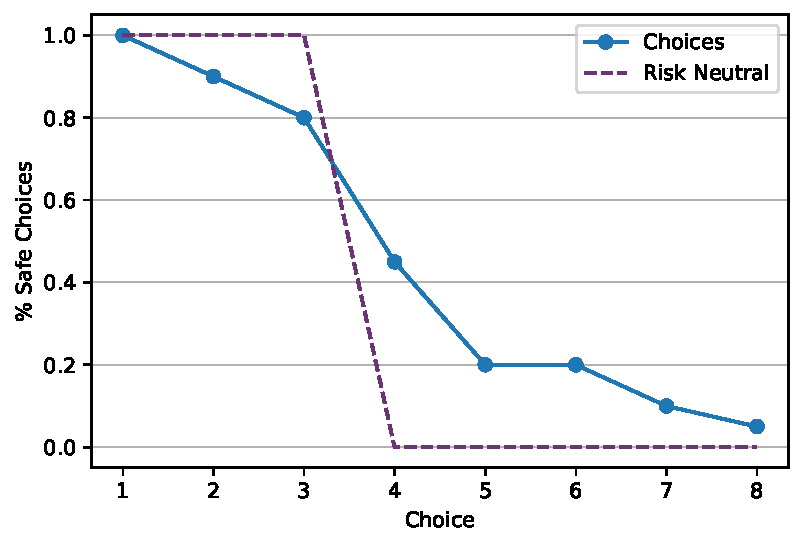
\includegraphics{graphics/aggregate_plot.pdf}
  \caption{Choices of sample versus risk averse choices}
\end{figure}











\subsection{Implementation}
The experiment was implented in oTree \textcite{chen_otreeopen-source_2016}, which is an open source framework for designing economics experiments. It is based on Python, and uses Django to create a front-end for users to participate in experiments. 

\textcite{holzmeister_otree_2017} made an implementation of the \textcite{holt_risk_2002} MPL in oTree which has been used as a resource(??)

The code for this project is available on GitHub \footnote{GitHub repository: \url{https://github.com/olafghanizadeh/hl_mpl}.}

\subsection{Deployment}


 

\newpage 
\section{Conclusion}




\printbibliography

\end{document}







